En este cap\'{i}tulo se aborda los conceptos necesarios que se necesita para comprender la detecci\'{o}n de anomal\'{i}as, as\'{i} tambi\'{e}n se expondr\'{a} los diferentes proyectos e investigaciones enfocados en la detecci\'{o}n de anomal\'{i}as de conducci\'{o}n. 
 
\section{Detecci\'{o}n de nomal\'{i}as}

Para comprender lo que implica la detecci\'{o}n de anomal\'{i}as, es necesario asimilar lo que \'{e}s una anomal\'{i}a y de que maneras estas pueden presentarse. Por lo tanto, se puede decir que las \textbf{anomalías}, o valores at\'{i}picos, son patrones en los datos que no se ajustan a una noción bien definida de un comportamiento normal.

\vspace{5mm} %5mm vertical space

Las anomal\'{i}as pueden ser clasificadas dentro de una de las tres siguientes categor\'{i}as:

\begin{enumerate}[1.]

\item \textbf{Anomal\'{i}as de punto: }Las anomalías de punto son simplemente instancias únicas y anómalas dentro de un conjunto de datos más grande, es decir, \'{e}stas se encuentran separadas del resto de los datos. Por ejemplo, en la Figura \ref{fig:anom_2D}, los puntos $o_1$, $o_2$ y la regi\'{o}n $O_3$ se encuentran fuera de los l\'{i}mites de las regiones normales ($N_1$ y $N_2$), y por lo tanto son anomal\'{i}as puntuales debido a que son diferentes al conjunto de datos normales.

\begin{figure}[h!]
  \begin{center}	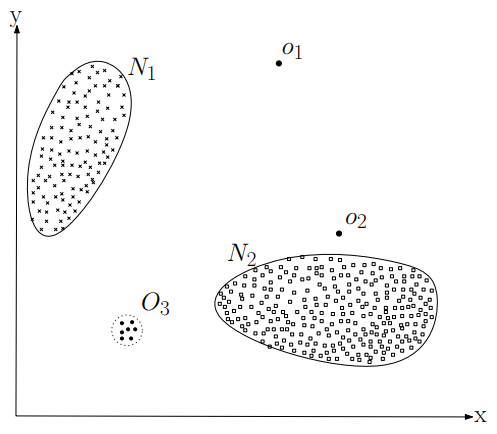
\includegraphics[width=0.45\textwidth]{imagenes/anom_2D}
  \caption{Ejemplo de anomal\'{i}as de punto en un conjunto de datos de 2 dimensiones.}
  \label{fig:anom_2D}
  \end{center}
\end{figure}

\vspace{5mm} %5mm vertical space

Este tipo de anomal\'{i}a se considera la m\'{a}s simple y es el foco de la mayor\'{i}a de las investigaciones enfocadas en la detecci\'{o}n de valores at\'{i}picos.

\item \textbf{Anomal\'{i}as contextuales (o condicionales): }Estos son puntos que s\'{o}lo se consideran anómalos en un contexto espec\'{i}fico. La noci\'{o}n de este contexto es inducida por la estructura en el conjunto de datos y debe especificarse como parte de la formulaci\'{o}n del problema.

\vspace{5mm} %5mm vertical space

Este tipo de anomal\'{i}as se han explorado con mayor frecuencia en los datos de series de tiempo y datos espaciales. La figura \ref{fig:anom_contx} muestra un ejemplo de serie temporal de la temperatura mensual de un \'{a}rea en los \'{u}ltimos 5 a\~{n}os, se debe tener en cuenta que la temperatura en el tiempo $t_1$ es la misma que en el tiempo $t_2$, pero se produce en un contexto diferente, por lo tanto $t_2$ es considerada una anomal\'{i}a.

\begin{figure}[h!]
  \begin{center}	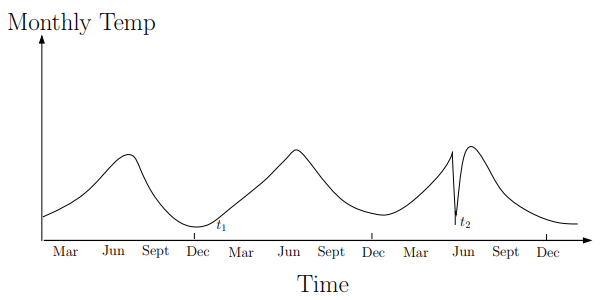
\includegraphics[width=0.6\textwidth]{imagenes/anom_contx}
  \caption{Anomal\'{i}a contextual $t_2$ en una serie temporal de temperatura.}
  \label{fig:anom_contx}
  \end{center}
\end{figure}

\item \textbf{Anomal\'{i}as colectivas: }
Si una colección de instancias de datos relacionadas es anómala con respecto a todo el conjunto de datos, se denomina anomalía colectiva.  Las instancias de datos individuales en una anomalía colectiva pueden no ser anomalías por sí mismas, pero su aparición conjunta como una colección es anómala.

\vspace{5mm} %5mm vertical space

La figura \ref{fig:anom_col} ilustra un ejemplo que muestra una salida de electrocardiograma humano, se puede notar que la región resaltada en rojo denota una anomalía porque existe el mismo valor bajo durante un tiempo anormalmente prolongado (que corresponde a una Contracción prematura auricular). Se debe tener en cuenta que ese valor bajo por sí mismo no es considerada una anomalía.

\begin{figure}[h!]
  \begin{center}	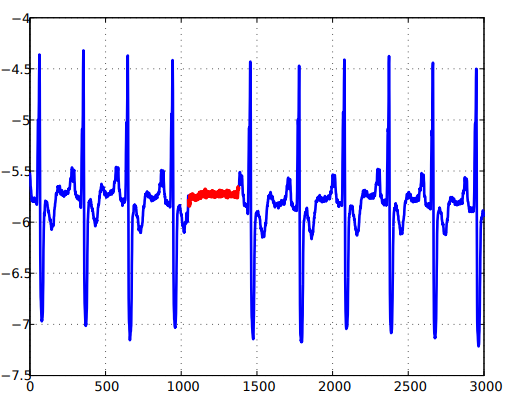
\includegraphics[width=0.45\textwidth]{imagenes/anom_col}
  \caption{Anomalía colectiva correspondiente a una contracción prematura auricular en un electrocardiograma humano.}
  \label{fig:anom_col}
  \end{center}
\end{figure}

\end{enumerate}

En relaci\'{o}n a lo expuesto previamente se puede definir como \textbf{detecci\'{o}n de anomal\'{i}as}, \'{o} \textbf{valores at\'{i}picos}, a la identificación de puntos de datos, elementos, observaciones o eventos que no se ajustan al patrón esperado de un grupo determinado. 

\vspace{5mm} %5mm vertical space

La detecci\'{o}n de anomal\'{i}as, se usa en distintos dominios de aplicaciones, por ejemplo: procesamiento de im\'{a}genes, detecci\'{o}n de fraudes de tarjeta, sistemas de detecci\'{o}n de intrusion de red, \'{e}tcetera.

\section{Desaf\'{i}os en la detecci\'{o}n de anomal\'{i}as}

En un nivel abstracto, la detecci\'{o}n de anomal\'{i}as puede parecer una tarea simple. Sin embargo puede llegar a ser una tarea muy desafiante. A continuaci\'{o}n se presenta algunos de estos desaf\'{i}os.

\begin{itemize}
\item La definici\'{o}n de regiones normales es bastante dif\'{i}cil. En muchos casos, los l\'{i}mites entre las anomal\'{i}as y los datos normales no son precisos. Por lo tanto, las observaciones normales podr\'{i}an considerarse anomal\'{i}as y viceversa.

\item Lo que se considera normal hoy en d\'{i}a, puede no ser normal en el futuro.

\item La mayor parte de las veces los enfoques para la detecci\'{o}n de anomal\'{i}as en un campo en espec\'{i}fico no se pueden utilizar en otro campo.

\item La poca disponibilidad de ejemplos positivos (anomal\'{i}as) para el entrenamiento y validaci\'{o}n del modelo de detecci\'{o}n de anomal\'{i}as.

\end{itemize}

\subsection{Enfoques de detecci\'{o}n de anomal\'{i}as}

Los enfoques que se pueden usar para este prop\'{o}sito se clasifican en las siguientes categor\'{i}as:

\subsubsection{Detecci\'{o}n de anomal\'{i}as supervisada}

El uso de t\'{e}cnicas de aprendizaje supervisado requiere la disponibilidad de un conjunto de datos de entrenamiento etiquetados, tanto para clases normales como an\'{o}malas. El enfoque principal es construir un modelo predictivo para clases normales vs. anomal\'{i}as, posteriormente tomar cualquier instancia de datos no visto, comparar con el modelo y determinar a que clase pertenece.

\vspace{5mm} %5mm vertical space

Existen dos principales inconvenientes que surgen con el uso de \'{e}sta t\'{e}cnica.

\begin{itemize}
\item La cantidad de instancias an\'{o}malas es muy inferior a la de las instancias normales, lo que genera un desequilibrio de distribuci\'{o}n de clases durante el entrenamiento.
\item La obtenci\'{o}n de etiquetas precisas y representativas, en particular para la clase de anomal\'{i}a, es un desaf\'{i}o.
\end{itemize}

\subsubsection{Detecci\'{o}n de anomal\'{i}as semi-supervisada}

Estas t\'{e}cnicas requieren un conjunto de entrenamiento con instancias etiquetadas, pero solo para la clase normal, esto hace que su uso sea m\'{a}s aplicable que las t\'{e}cnicas supervisadas, ya que no se requiere etiquetas para la clase anomal\'{i}a.

\vspace{5mm} %5mm vertical space

El enfoque típico usado en \'{e}stas técnicas es construir un modelo para la clase correspondiente al comportamiento normal, y usar el modelo para identificar anomalías en los datos de prueba.

\subsubsection{Detecci\'{o}n de anomal\'{i}as no supervisada}

Las t\'{e}cnicas que operan de manera no supervisada no requieren datos de entrenamiento, raz\'{o}n por la cual son las m\'{a}s ampliamente utilizadas. Estas t\'{e}cnicas suponen que las instancias normales son mucho m\'{a}s frecuentes que  las anomal\'{i}as en los datos de prueba, en caso de que esta suposici\'{o}n no sea cierta, tales t\'{e}cnicas sufren de una alta tasa de falsas alarmas.

\section{Trabajo relacionado}

La identificación de comportamientos de conducción anormal es una parte indispensable para mejorar la seguridad de conducción, sin embargo, como se vi\'{o} previamente, \'{e}sta no es una tarea sencilla. En los últimos años, se han propuesto varias técnicas para detectar conductas de manejo. Esta secci\'{o}n esta dedicada al repaso de las mismas.

\vspace{5mm} %5mm vertical space

Dang-Nhac et al. \cite{20}, proponen un sistema combinado que se compone de dos módulos: uno para detectar el tipo de vehículo de los usuarios y el otro para detectar los eventos de conducción instantánea, independientemente de la orientación y la posición de los teléfonos inteligentes, \'{e}ste sistema logra una precisión promedio del 98.33\% en la detección del tipo del vehículo (autom\'{o}vil, motocicleta, bicicleta, entre otros) y una precisión promedio de 98.95\% en el reconocimiento de los eventos de conducción de los motociclistas al usar Random Forest como clasificador .

\vspace{5mm} %5mm vertical space

Por otra parte en \cite{21} Ferreira et al. presentan una evaluación cuantitativa de 4 Algoritmos de Aprendizaje Autom\'{a}tico ( Bayesian Network BN, Artificial Neural Network ANN, Random Forest RF y Support Vector Machine SVM) con diferentes configuraciones, aplicadas en la detección de 7 tipos de eventos de conducción, entre eventos normales y agresivos, utilizando datos recopilados de 4 sensores de teléfonos inteligentes Android (acelerómetro, aceleración lineal, magnetómetro y giroscopio); dando como resultado que el giroscopio y el acelerómetro son los mejores sensores para detectar eventos de conducción y que Random Forest (RF) es por lejos el Algoritmo de Aprendizaje Autom\'{a}tico de mejor rendimiento, seguido de la forma m\'{a}s simple de ANN el Multi Layer Perceptron (MLP).

\vspace{5mm} %5mm vertical space

En \cite{23} proponen el sistema MIROAD el cual muestra que el Dynamic Time Warping (DTW) es un algoritmo válido para detectar maniobras de conducción potencialmente agresivas, donde casi todos los eventos agresivos (97\%) se identificaron correctamente, utilizando el conjunto de sensores T (aceler\'{o}metro, giroscopio y el tono de voz). As\'{i} tambi\'{e}n en \cite{24} se propone un sistema enfocado a desarrollar la conciencia del conductor mediante notificaciones en situaciones críticas que pueden desencadenar maniobras de manejo inseguras, mediante un modelo para detectar situaciones peligrosas basadas en Object-Oriented Bayesian Network (OOBN).

\vspace{5mm} %5mm vertical space

As\'{i} como los trabajos presentados previamente existe gran cantidad de trabajos (\cite{25}, \cite{26}, \cite{27}, \cite{28}, \cite{29}) que usan los sensores de los tel\'{e}fonos inteligentes (aceler\'{o}metro y giroscopio) para la detecci\'{o}n de conducci\'{o}n agresiva, esto debido a que se tiene la ventaja de no comprar ni instalar ning\'{u}n dispositivo y adem\'{a}s de ser altamente portatil, sin embargo se depende bastante del rendimiento del receptor GPS y no es aplicable en \'{a}reas no disponibles para GPS.

\vspace{5mm} %5mm vertical space

Existen adem\'{a}s otros enfoques para la detecci\'{o}n de conducci\'{o}n agresiva de un conductor, por ejemplo en \cite{22} proponen un método basado en Convolutional Neural Network (CNN) para detectar la emoción de conducción agresiva, mediante la utilizaci\'{o}n de imágenes faciales de un conductor obtenidas con una cámara de luz NIR y una cámara térmica.

\section{Enfoque sobre el problema}

Es evidente que \'{e}ste tema fue ampliamente investigado y que tiene una gran variedad de propuestas de soluci\'{o}n, sin embargo la mayor\'{i}a de estas se basan en la detecci\'{o}n mediante t\'{e}cnicas de aprendizaje supervisado, lo cual presenta la gran desventaja de requerir datos etiquetados para generar el modelo de detecci\'{o}n; adem\'{a}s gran parte de los trabajos relacionados proponen modelos generalizados para la detecci\'{o}n y no as\'{i} modelos espec\'{i}ficos por usuarios, lo cual es crucial debido a que cada conductor presenta conductas individuales de manejo y manejan en condiciones distintas, es decir, la conducci\'{o}n de un usuario que circula por avenidas pavimentadas ser\'{a} distinta a la conducci\'{o}n de un usuario que circula por calles empedradas o la conducci\'{o}n de un usuario que circula por avenidas o calles concurridas ser\'{a} distinta a de los usuarios que circulen por calles relativamente descongestionadas.

\vspace{5mm} %5mm vertical space

Por las razones enunciadas anteriormente el presente proyecto propone un m\'{e}todo de detecci\'{o}n de anomal\'{i}as de conducci\'{o}n (Figura \ref{fig:metodo}) como alternativa a las ya existentes.

\begin{figure}[h!]
  \begin{center}	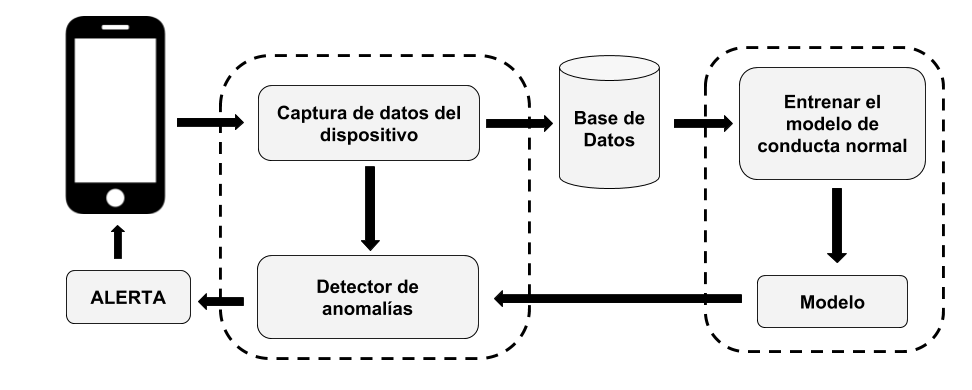
\includegraphics[width=0.85\textwidth]{imagenes/metodo}
  \caption{M\'{e}todo de detecci\'{o}n propuesto.}
  \label{fig:metodo}
  \end{center}
\end{figure}

\vspace{5mm} %5mm vertical space

Este m\'{e}todo se compone de las siguientes partes principales:

\vspace{5mm} %5mm vertical space

\begin{itemize}
\item Captura y an\'{a}lisis de datos.
\item Generaci\'{o}n del modelo de conducta normal de conducci\'{o}n.
\item Detector de anomal\'{i}as.
\end{itemize} 

Los cuales ser\'{a}n abordados en los siguientes capitulos.

\section{Resumen del cap\'{i}tulo}

De acuerdo a los conceptos presentados acerca de la detecci\'{o}n de anomal\'{i}as, los desaf\'{i}os  que presenta la detecci\'{o}n de las mismas y los trabajos de investigaci\'{o}n realizados en este campo hasta la fecha, se propone un m\'{e}todo de detecci\'{o}n de anomal\'{i}as de conducci\'{o}n mediante el uso de t\'{e}cnicas de Aprendizaje Autom\'{a}tico y el uso de un dispositivo m\'{o}vil, los mismos ser\'{a}n tratados en profundidad en los siguientes cap\'{i}tulos. 